\subsection{Performance of Interference Aware Job Scheduling Algorithm}


To evaluate the performance of the job scheduling algorithm, we used the four Apache Spark jobs as before (e.g., PageRank (PR), K-Means (KM), Logistic Regression (LR) and WordCount (WC)). The order of job submission was varied in different experiments and the submission time was randomly chosen between 0 to 100 sec. The performance of our algorithm is compared against the default condition where each job is started immediately after submission. 

\noindent
In the first experiment, the four jobs were submitted in the order of PR, KM, LR, WC, and the input data size was set to 20GB for each of them. PR was submitted at $0s$, KM was submitted at $16s$, LR was submitted at $47s$, and WC was submitted at $94s$. As shown in Figure \ref{exp1}, the average execution time of individual jobs and total execution time (i.e., completion time of the last job minus the start time of the first job) were reduced by 47\% and 10\% respectively. 



\noindent
In the second experiment, the four jobs were submitted in the same order (PR, KM, LR, WC), but the input data size were set to 20GB for PR, 15GB for KM, 10GB for LR and 5GB for WC. PR was submitted at $0s$, KM was submitted at $59s$, LR was submitted at $88s$, and WC was submitted at $97s$. As shown in Figure \ref{exp2}, the average execution time of individual jobs and total execution time were reduced by 34\% and 13\% respectively. 

\noindent
In the third experiment, the four jobs were submitted in the order of KM, WC, PR, LR, and the input data size were set to 10GB for KM, 20GB for WC, 15GB for PR and 5GB for LR respectively. KM was submitted at $0s$, WC was submitted at $30s$, PR was submitted at $51s$, and LR was submitted at $71s$. As shown in Figure \ref{exp3}, the average execution time of individual jobs and total execution time were reduced by 26\% and 2\% respectively. 

\noindent
In the fourth experiment, the four jobs were submitted in the order of LR, WC, KM, PR, and the input data size were set to 15GB for LR, 10GB for WC, 20GB for KM and 15GB for PR respectively. LR was submitted at $0s$, WC was submitted at $8s$, KM was submitted at $53s$, and PR was submitted at $64s$. As shown in Figure \ref{exp4}, the average execution time of individual jobs and total execution time were reduced by 39\% and 8\% respectively. 

\noindent
In the fifth and last experiment, the four jobs were submitted in the order of WC, PR, LR, KM, and the input data size were set to 20GB for WC, 15GB for PR, 10GB for LR and 10GB for KM respectively. WC was submitted at $0s$, PR was submitted at $7s$, LR was submitted at $27s$, and KM was submitted at $71s$. As shown in Figure \ref{exp5}, the average execution time of individual jobs and total execution time were reduced by 40\% and 8\% respectively. 


\begin{figure}[!t]
\centering
\captionsetup{justification=centering}
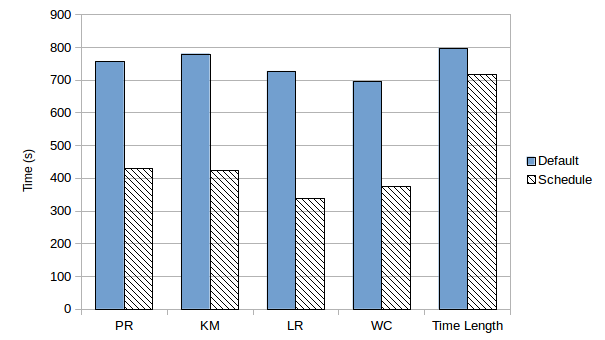
\includegraphics[width=3in]{exp1.png}
\caption{Result of Scheduling Experiment 1. Column Time length represents the total execution time (completion time of the last job minus the start time of the first job).}
\label{exp1}
\end{figure}

\begin{figure}[!t]
\centering
\captionsetup{justification=centering}
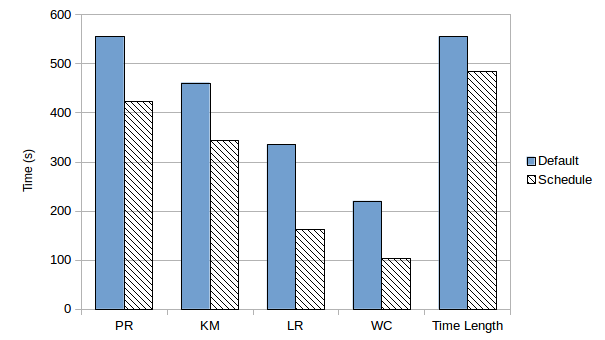
\includegraphics[width=3in]{exp2.png}
\caption{Result of Scheduling Experiment 2. Column Time length represents the total execution time (completion time of the last job minus the start time of the first job).}
\label{exp2}
\end{figure}

\begin{figure}[!t]
\centering
\captionsetup{justification=centering}
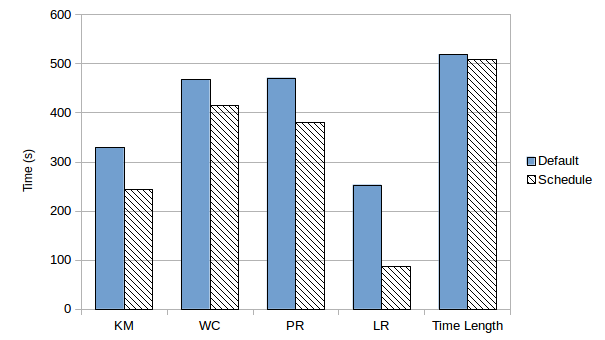
\includegraphics[width=3in]{exp3.png}
\caption{Result of Scheduling Experiment 3. Column Time length represents the total execution time (completion time of the last job minus the start time of the first job).}
\label{exp3}
\end{figure}



\begin{figure}[!t]
\centering
\captionsetup{justification=centering}
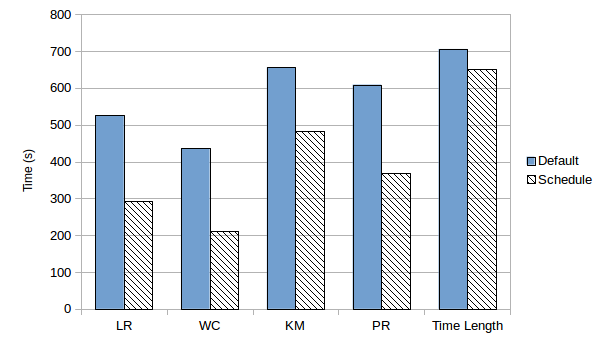
\includegraphics[width=3in]{exp4.png}
\caption{Result of Scheduling Experiment 4. Column Time length represents the total execution time (completion time of the last job minus the start time of the first job).}
\label{exp4}
\end{figure}





\begin{figure}[!t]
\centering
\captionsetup{justification=centering}
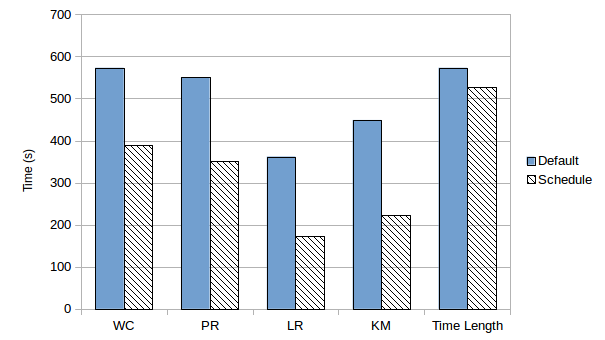
\includegraphics[width=3in]{exp5.png}
\caption{Result of Scheduling Experiment 5. Column Time length represents the total execution time (completion time of the last job minus the start time of the first job).}
\label{exp5}
\end{figure}

